\documentclass[12pt]{article}
\usepackage[papersize={8.5in,11in}]{geometry}
\usepackage[pdftex]{graphicx}
\DeclareGraphicsExtensions{.pdf,.png,.jpg}
%
\usepackage{amsmath}
\usepackage{amsthm}
\usepackage{amssymb}
\usepackage{textcomp}
\usepackage[all]{xy}
\usepackage{fancyhdr}
\usepackage{hyperref}
\usepackage{verbatim}
\usepackage{algorithm}
\usepackage{algorithmic}
\usepackage{color}
\usepackage[usenames,dvipsnames,svgnames,table]{xcolor}
\usepackage{rotating}
\usepackage{wrapfig}
\usepackage{tikz}
\usetikzlibrary{shapes.geometric, arrows}
\usepackage{framed}
\usepackage[scaled=0.75]{FiraMono}
%\usepackage{newtxtt}

\usepackage{listings}
\lstset{language=python,frame=ltrb,framesep=5pt,basicstyle=\ttfamily,
 keywordstyle=\ttfamily\color{DarkRed}\bfseries,
%morecomment=[n][\textbf]{In\ [}{]\:},
%morecomment=[n][\textbf]{Out\ [}{]\:},
morecomment=[s][\color{blue}]{In\ [}{]\:},
morecomment=[s][\color{red}]{Out[}{]\:},
identifierstyle=\ttfamily\color{DarkBlue},
commentstyle=\color{OliveGreen},
stringstyle=\ttfamily\color{Orange},
showstringspaces=false,tabsize = 3}

\lstdefinelanguage{shell} {
commentstyle = \color{black},
keywordstyle = \color{black},
stringstyle = \color{black},
identifierstyle = \color{black},
morecomment=[s][\color{blue}]{In\ [}{]\:},
morecomment=[s][\color{red}]{Out[}{]\:},
 }


%
% this gives a little box for the end of a proof:
%
\def\endthrmbox{$\sqsubset \!\!\!\! \sqsupset$}

\newcommand{\dis}{\displaystyle}
 \def      \RR             {{\mathbb R}}
        \def      \NN             {{\Bbb N}}
        \def      \QQ             {{\Bbb Q}}
        \def      \CC             {{\Bbb C}}
        \def      \ZZ             {{\Bbb Z}}


        \def       \a              {{\alpha}}
        \def       \b              {{\beta}}
        \def       \d              {{\delta}}
        \def       \D              {{\Delta}}
        \def         \e              {{\varepsilon}}
        \def         \g              {{\gamma}}
        \def         \G              {{\Gamma}}
        \def       \l              {{\lambda}}
        \def       \L              {{\Lambda}}
        \def        \m               {{\mu}}
        \def         \n              {{\nabla}}
        \def       \var          {{\varphi}}
        \def         \s              {{\sigma}}
        \def       \Sig          {{\Sigma}}
        \def       \Om          {{\Omega}}

        \def       \t              {{\tau}}
        \def         \th             {{\theta}}
        \def       \O              {{\Omega}}
        \def       \o              {{\omega}}
        \def         \z              {{\zeta}}
       \def        \P             {{\Phi}}
       \def        \p             {{\phi}}
        %Other macros

        \def       \iy              {{\infty}}
        \def         \pa             {{\partial}}
        \def         \div           {{\rm div}}
         \def       \na            {{\nabla}}


%\renewcommand\baselinestretch{1.3}
%% The following block is for narrow margins:
\setlength{\topmargin}{-0.9in}
\setlength{\textheight}{9.50in}
\setlength{\oddsidemargin}{-0.375in}
\setlength{\evensidemargin}{-0.375in}
\setlength{\textwidth}{7.25in}
\setlength{\parindent}{0pt}
\setlength{\parskip}{2pt}
%% end page descript.




\usepackage[compact,explicit]{titlesec}
\titleformat{\section}[runin]{\large\bfseries}{}{0pt}{\titlerule[1.5pt]\newline\vspace*{-4pt}\quad
\newline}%[\vspace{0.01ex}{\titlerule[1.5pt]}]

\usepackage[final]{pdfpages}


\title{Homework \#2}
\author{Kyle MacMillan, \\Remmington Bullis}


\begin{document}
\maketitle

% Any information we want to say upfront
The repository for this paper is \href{https://github.com/macattackftw/ncGA}{here}. 
The \texttt{README.md} contains a gif of our solution in action.

\section{} %%  This will generate a numbered problem header.

\subsection{Statement}
Problem statement.

\subsection{Method}


\newpage
\subsection{Results}
Our results.

\begin{figure}[H]
\centering
\noindent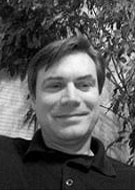
\includegraphics[width=0.65\textwidth]{./images/jmcgough}
\caption{The Persistence of Memory}
\label{fig:jmcgough}
\end{figure}

\begin{figure}[H]
\centering
\noindent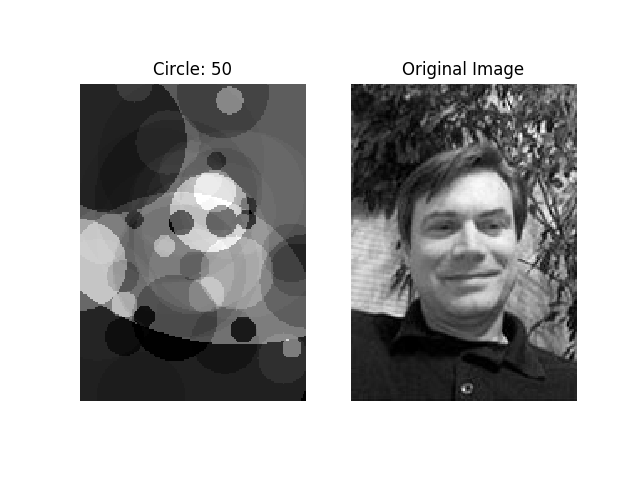
\includegraphics[width=0.65\textwidth]{./results/jmcgough_050}
\caption{\textit{The Persistence of Memory} with 50 circles}
\label{fig:jmcgough_050}
\end{figure}

\begin{figure}[H]
\centering
\noindent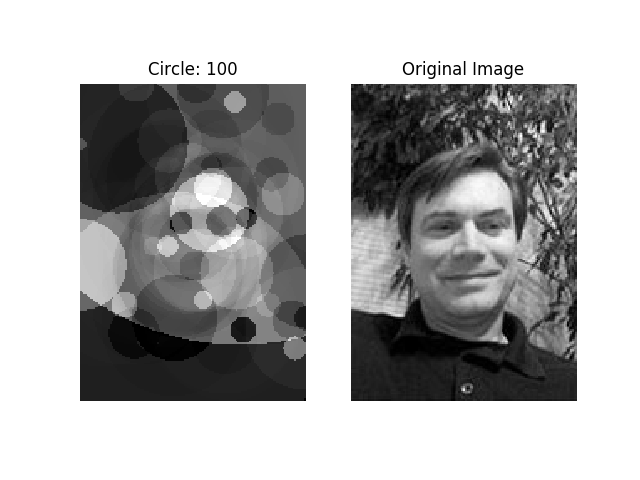
\includegraphics[width=0.65\textwidth]{./results/jmcgough_100}
\caption{\textit{The Persistence of Memory} with 100 circles}
\label{fig:jmcgough_100}
\end{figure}

\begin{figure}[H]
\centering
\noindent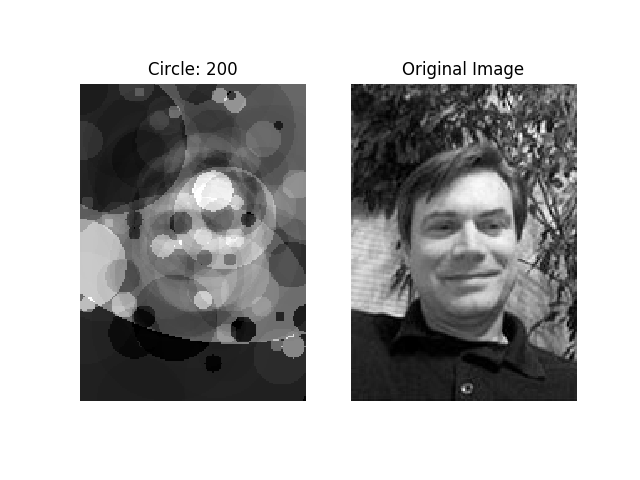
\includegraphics[width=0.65\textwidth]{./results/jmcgough_200}
\caption{\textit{The Persistence of Memory} with 200 circles}
\label{fig:jmcgough_200}
\end{figure}



\newpage
\subsection{Code}
\subsubsection{Best Circle}
\begin{lstlisting}
import numpy
\end{lstlisting}


\end{document}
